% SPDX-License-Identifier: CC-BY-4.0
% Copyright (c) 2026 Jonathan Yantis. Research draft; not submitted.
\documentclass[11pt,letterpaper]{article}
\usepackage[margin=0.85in]{geometry}
\usepackage[T1]{fontenc}
\usepackage{mathptmx,amsmath,amssymb,booktabs,array,ragged2e,xcolor,microtype,xurl,hyperref,fancyhdr,longtable,pgfplots}
\pgfplotsset{compat=1.18}
\definecolor{studyblue}{RGB}{39,83,109}
\definecolor{studyorange}{RGB}{180,94,32}
\hypersetup{colorlinks=true,urlcolor=studyblue,citecolor=studyblue,linkcolor=black,pdfauthor={Jonathan Yantis},pdftitle={How Much Timing Information Is Enough? Awake Hardware Evidence and Wake/Listen Energy Models for PToB}}
\setlength{\parindent}{1em}\setlength{\parskip}{3pt}\setlength{\headheight}{14pt}\setlength{\emergencystretch}{2em}
\widowpenalty=10000\clubpenalty=10000
\renewcommand{\floatpagefraction}{0.8}\renewcommand{\topfraction}{0.9}\renewcommand{\textfraction}{0.1}
\pagestyle{fancy}\fancyhf{}\fancyhead[L]{\small PToB Wake/Listen Scheduling}\fancyhead[R]{\small Research draft, 19 October 2026}\fancyfoot[C]{\small\thepage}
\newcommand{\ns}{\,\mathrm{ns}}\newcommand{\us}{\,\mu\mathrm{s}}\newcommand{\ms}{\,\mathrm{ms}}\newcommand{\ppm}{\,\mathrm{ppm}}
\newcommand{\code}[1]{\texttt{#1}}
\newcolumntype{L}[1]{>{\RaggedRight\arraybackslash}p{#1}}
\begin{document}
\title{\vspace{-1.2em}How Much Timing Information Is Enough?\\Awake Hardware Evidence and Wake/Listen\\Energy Models for PToB}
\author{Jonathan Yantis\\\small Independent researcher}
\date{19 October 2026\\\small Research draft for possible arXiv submission; not submitted or peer reviewed}
\maketitle
\begin{abstract}
Precision Time over BLE (PToB) can estimate a clock from hardware event timestamps even when their completed references arrive later. This raises a power question: how little new timing information could sustain useful precision between listens? We report an awake hardware pilot on one T096 receiver, with six randomized 20-window runs using 125 ms training windows and 5, 10 or 20 s HOLD intervals. A fixed acquisition-derived phase anchor aligned every window; both receive capture and completed reference had to fit. All schedules completed, but only 42 of 120 windows refreshed the fit. Of 78 empty windows, 69 contained no accepted timing pairs and nine had reception without a complete selected pair. Per-run causal HOLD BLE RMS after an inherited fixed normalization was 98--333 ns; its observation coverage was strongly incomplete in several runs. Independently observed, eligible local PPS fractional-phase RMS was 80--2174 ns, with 1400/1400 recorded HOLD edges eligible. Only one run replaced all 16 acquisition fit pairs, leaving 10.17 s of post-turnover observation. Radio reception and the precision counter remained active throughout. Consequently, scheduled training fractions of 2.439\%, 1.235\% and 0.621\% establish neither radio duty cycle nor energy savings. We derive explicit complete-pair, guard, drift, wake-overhead and reacquisition models, examine sub-1/10/100 $\mu$s RMS targets, and specify physical sleep and power experiments needed to test the potential. A sanitized supplement reproduces the reported derived-data results offline while preserving failures, missing observations and separate source populations.
\end{abstract}
\noindent\small Copyright \copyright\ 2026 Jonathan Yantis. Original manuscript and figures: \href{https://creativecommons.org/licenses/by/4.0/}{CC BY 4.0}. Executable analysis: MIT.\normalsize

\section{Introduction}
Time synchronization need not require a continuously changing estimate. A receiver with an adequate local frequency estimate may project time between occasional updates. The useful scheduling question is therefore not simply how many packets arrive, but how often a complete, admissible timing relation arrives early enough to improve a retained clock model. Radio startup, reference completion, fit history, source outages and the survival of the timebase across sleep all affect that answer.

PToB explores authenticated timing over Bluetooth Low Energy periodic advertising. A received event has a local hardware capture; a subsequently completed reference associates it with source time. An affine map converts the receiver counter to an experimental source-clock estimate. Restricting which pairs may train that map lets an awake receiver emulate a limited information budget while continuing to observe its prediction error. The counterfactual is limited: a physically sleeping receiver may lose the oscillator, transport synchronization, authentication context or event capture behavior that made the awake prediction possible.

This paper contributes three things. First, it documents a finite hardware information-budget pilot with a fixed, acquisition-only phase anchor, hard completion apertures, frozen HOLD states and complete window accounting. Second, it connects measured pair availability and fit turnover to explicit scheduling and hypothetical energy equations, without treating model inputs as measured power. Third, it provides public derived observations, claim provenance and a concrete protocol for retained-counter idle, low-frequency-clock sleep, radio reacquisition and physical reset experiments.

The central finding is mixed. Phase alignment positioned selected pairs comfortably within 125 ms windows, and the observed conditional relative precision often met a sub-microsecond RMS target. Yet several runs lost most BLE observation coverage, and five of six never replaced their acquisition history. A low conditional RMS during a long gap does not demonstrate reliable sparse maintenance. The next experiment must establish both the energy saved and the clock information that survives actual sleep.

\section{Prior work and platform constraints}\label{sec:prior}
Reference Broadcast Synchronization separates event observations from sender-side delivery uncertainty using common broadcasts \cite{rbs}. FTSP combines MAC-layer timestamps with skew estimation and periodic flooding \cite{ftsp}. These establish relevant principles: timestamping the physical event and estimating relative frequency can reduce dependence on software delivery timing. The present contribution is narrower than a new synchronization primitive: it studies the completion aperture, missingness and retained-fit cost of a particular BLE implementation under a sparse information gate. No precision ranking against those systems is attempted; their platforms, topology and endpoints differ.

Bluetooth Core 6.0 describes periodic advertising trains and acquisition of their synchronization information, and its Link Layer window-widening rules account for clock uncertainty since synchronization \cite{btcore}. A known periodic interval alone does not ensure a complete PToB pair. This experiment's 62.5 ms packet grid, 8 ms lead and host-visible completion rule are implementation and treatment parameters. They are not a Bluetooth guarantee that an application can stop the radio for 20 s and retain its train or admission.

Nordic's nRF52840 power documentation distinguishes System ON from System OFF, configurable RAM retention, and reset on wake from System OFF \cite{nordicpower}. The clock documentation states that LFCLK is stopped in System OFF and that the synthesized LF source depends on HFCLK \cite{nordicclock}. The RTC can operate from LFCLK while HFCLK is off, with a base counter resolution of about 30.517 $\mu$s \cite{nordicrtc}. These are SoC mechanisms, not measurements of the T096 board. Retaining RAM does not by itself preserve a running precision counter or establish time elapsed while the clocks were stopped.

Zephyr system power management requires an appropriate wake event and platform-supported states; its residency policy accounts for both minimum residency and exit latency \cite{zephyrsystem}. Device runtime power management separately manages device usage and suspension \cite{zephyrruntime}. An application timeout or a sleeping thread does not prove that Bluetooth, USB, clocks, GNSS, display or their regulators reached the intended power state. No new sleep processor or Zephyr power-management integration is implemented or validated here.

\section{Experimental clock and measurement definitions}\label{sec:definitions}
\subsection{The awake PC image}
The Power Control (PC) image is a separate, flash-only BLE leaf experiment. It is distinct from ordinary grandmaster (GM) and relay-clock (RC) mesh profiles and from the GNSS/USB Direct Connect (DC) image. PC117 is firmware 0.15.117 at source checkpoint
\begin{center}\small\code{9ee2bcbc7cdd7bf27e6da80fb65aabf47ff04606}.\end{center}
It retains the awake precision counter and synthesized-LF configuration, authenticated receiver and continuous causal observations. It gates training during HOLD; it does not implement physical sleep. The experiment does not qualify GM, RC, DC, USB time delivery or normal output permissions.

Let $c$ be the receiver counter and let a retained map be
\begin{equation}
 \widehat{t}(c)=a+b(c-c_0).\label{eq:map}
\end{equation}
The selected 16-pair rolling estimator may carry acquisition pairs across several windows. HOLD freezes its training count, map generation and rate. This experimental arithmetic projection may outlive ordinary permission to publish time. Source, map, authentication and session expiry remain independent constraints; an experimental phase estimate is not renewed timing authority.

\subsection{Causal BLE error, bias and missingness}
A causal BLE record scores a captured RX against the preceding map before training on the new completed pair. A late description of the event is not used to retroactively improve that event's prediction. We retain raw signed error $e_i$ and the inherited provisional normalization
\begin{equation}
 e_i^{\mathrm{norm}}=e_i+10543\ns,\qquad
 R=\sqrt{\frac{1}{n}\sum_{i=1}^{n}(e_i^{\mathrm{norm}})^2}.\label{eq:rms}
\end{equation}
The constant was not estimated from these six runs; its calibration and portability are not established. There is no run-specific fitted bias, detrending or mean removal. The supplement also reports raw RMS, signed means and maxima. The sub-microsecond BLE statements below refer to the normalized residual, not uncorrected absolute timing accuracy.

The denominator $n$ includes only valid recorded samples in the stated run and HOLD phase. Invalid and out-of-run records remain in the export with their flags. No observation is imputed during source loss. We additionally count occupied one-second HOLD bins, indexed separately within each cycle, out of $20H$ expected bins for integer-second $H$. A bin with one score is occupied; this is a coarse observation-coverage measure, not the fraction of continuous time for which precision or output is guaranteed. Empty bins are unknown.

\subsection{Independent PPS fractional phase}
The receiver also hardware-observes a local PPS witness that is not used to train the BLE map. Eligibility requires the recorded map-projection flag, reference seen, reference fix, reference PPS, a zero reason code, and the experimental projection flag during HOLD. Each recorded phase remains associated with its run and source scope. This is an independent observation path relative to the fit, not an independently calibrated UTC or electrical-output accuracy test. Reference association, fixed path bias, source-chain errors and PPS-to-UTC calibration remain unresolved. One PPS sample per second also cannot resolve subsecond excursions between edges.

A recorded HOLD edge being eligible means it supports the stated fractional-phase calculation. It does not prove that ordinary output was authorized or that all possible physical PPS edges were independently enumerated. We report recorded/eligible counts; the sealed capture audit found no logger cursor gaps in its recorded streams.

\section{Protocol, populations and integrity}\label{sec:protocol}
The main evidence is the closed PC117 collection selected on 19 October 2026 \cite{supplement}. The sealed private index has SHA-256
\begin{center}\footnotesize\code{7fad272ec1426dea568e8c323d6349f4fc686d676911fb60384abd265bf8a33d}.\end{center}
All 34 selected files and raw-capture, analysis and restoration manifests were checked. Independent re-extraction into a new directory reproduced the four derived CSV files byte for byte, and separate verifiers checked counts, RMS, apertures and frozen HOLD states. Checksums bind bytes; they do not establish accuracy, calibration or independent physical replication.

The treatment used one receiver (cohort alias TC-02), one physical boot, the operator's existing placement, and authenticated direct-GM selection. Actual source/root/boot/capture epochs were recorded privately and are represented publicly by equality-preserving scope aliases. B1 uses S01, B2--B5 use S02, and B6 uses S03 in valid observations. Even where the alias matches, runs retain separate priming fits and observation windows. No RMS is pooled across runs, firmware, geometry or epochs.

The predeclared schedule used random seed 2026101916: two repetitions each of 5, 10 and 20 s HOLD, each with 20 windows. Chronological order was 10/r1, 20/r1, 5/r2, 5/r1, 10/r2, 20/r2. A preliminary canary used three 125 ms windows separated by 1 s HOLD and selected two pairs. Priming used a 2 s logical-estimator listening budget with a retained awake counter and admitted receiver; it was not a physical boot. There were nine priming attempts including the canary: seven complete, two failed. Passive source waits after a failure were bounded at 180 s with at most two attempts per block. All six main schedules subsequently started and completed. Their completion is a scheduler result, not a statement that every window received information.

\subsection{Fixed aperture and anchor}
A completed authenticated pair in the acquisition scope supplied a single RX phase anchor. The 16 MHz counter schedule used packet period $P=62.5\ms$, guard $g=8\ms$, and at least 5 ms from command to the first window. For scheduled start $s_k$,
\begin{equation}
 s_k=s_1+(k-1)(W+H),\quad W=125\ms,\quad
 (s_1+g-c_{\mathrm{anchor}})\bmod P=0.\label{eq:schedule}
\end{equation}
Here the terms in the modular relation are converted to the same counter units. Neither off-window observations nor missed references rephase or widen a run. Admission for training requires
\begin{equation}
 s_k\le c_{\mathrm{RX}}\le c_{\mathrm{complete}}<s_k+W.\label{eq:aperture}
\end{equation}
A capture inside LISTEN whose reference completes after its deadline is excluded. A changed authenticated source scope fails the treatment and requires acquisition. The alignment audit examined 123 distinct HOLD cycle states: 120 main and three canary states, with frozen training count, generation and rate within each state.

The nominal scheduled training fraction is
\begin{equation}
 f_{\mathrm{train}}=\frac{W}{W+H}
 =\{2.439,1.235,0.621\}\%\quad\text{for }H=\{5,10,20\}\,\mathrm{s}.\label{eq:fraction}
\end{equation}
Radio reception stayed enabled to score HOLD behavior. This fraction measures the aperture made eligible for training. It is neither measured radio-on time, packet airtime, CPU duty cycle nor energy consumption.

\subsection{Earlier evidence remains separate}
Earlier PC112 logical-reset listening trials attempted 13 of 37 planned treatments: 12 completed, one was incomplete with no return, and 24 were unstarted. Their listening-budget and HOLD-bin summaries are retained as a separate contextual export, including empty bins; they are not additional PC117 replicates. In PC115, three 2 s logical-reset acquisition trials bracketed first-map availability about 0.538--0.655 s after the first completed pair, with ten training pairs at that first map. Two trials completed; the third did not return. Those brackets exclude physical startup and do not prescribe a cold-wake budget.

PC115's separate cadence population had six complete cases, six skipped for unavailable priming and one refused start. Its 125 ms/20 s case selected zero pairs in 16 windows; the constant projection continued for 322 s, with 320 eligible HOLD PPS observations and 2490.247 ns fractional-phase RMS. This is awake zero-refresh holdover, not evidence of successful sparse refresh. Earlier HOLD-window validation and PC112 initial-listening observations have different selections and denominators. PC116 was stopped by the investigator after one complete main block and an interrupted second block; four main blocks were unstarted. Extra discovery activity during deliberate held-map expiry motivated a PC-only change in PC117. Its contribution to the observed source loss remains unproved. These histories motivate controls; they are not pooled outcomes or explanations of PC117 outages.

\section{Measured PC117 results}\label{sec:results}
\subsection{Refresh availability and completion}
Table~\ref{tab:availability} lists each main run. There were 42 selected refreshes in 120 windows, with 78 empty windows. Of the empty windows, 69 contained no accepted timing pairs anywhere in that cycle and nine had accepted reception without a complete selected pair in the aperture. These are observation categories; ``no accepted pair'' does not identify the RF, source, admission or software cause of absence. A window can exclude a second late pair while still selecting an earlier complete pair. Excluded-pair counts therefore must not be interpreted as empty-window counts.

\begin{table}[t]
\centering\small
\caption{Main runs in chronological order. $H$ is HOLD seconds. ``No pairs'' counts whole cycles with no accepted timing pair. ``RX/no select'' is the remaining empty-window category. Map generations describe each run's retained fit.}\label{tab:availability}
\begin{tabular}{lrrrrrrr}\toprule
Run & $H$/rep & Selected & Empty & No pairs & RX/no select & Map gen. & Duration (s)\\\midrule
B1 & 10/1 & 4/20 & 16 & 15 & 1 & 24--28 & 202.5\\
B2 & 20/1 & 5/20 & 15 & 14 & 1 & 27--32 & 402.5\\
B3 & 5/2 & 16/20 & 4 & 0 & 4 & 26--42 & 102.5\\
B4 & 5/1 & 1/20 & 19 & 18 & 1 & 23--24 & 102.5\\
B5 & 10/2 & 10/20 & 10 & 8 & 2 & 23--33 & 202.5\\
B6 & 20/2 & 6/20 & 14 & 14 & 0 & 24--30 & 402.5\\\bottomrule
\end{tabular}
\end{table}

\begin{figure}[t]\centering
% BEGIN GENERATED window-outcomes
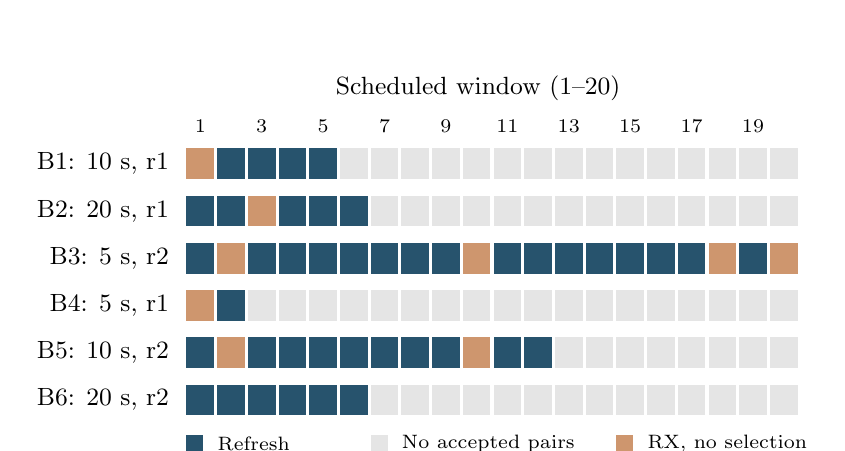
\begin{tikzpicture}[x=0.39cm,y=0.60cm]
\node[anchor=east,font=\small] at (-.25,5) {B1: 10 s, r1};
\fill[studyorange!65] (0,4.675) rectangle ++(.90,.65);
\fill[studyblue] (1,4.675) rectangle ++(.90,.65);
\fill[studyblue] (2,4.675) rectangle ++(.90,.65);
\fill[studyblue] (3,4.675) rectangle ++(.90,.65);
\fill[studyblue] (4,4.675) rectangle ++(.90,.65);
\fill[gray!20] (5,4.675) rectangle ++(.90,.65);
\fill[gray!20] (6,4.675) rectangle ++(.90,.65);
\fill[gray!20] (7,4.675) rectangle ++(.90,.65);
\fill[gray!20] (8,4.675) rectangle ++(.90,.65);
\fill[gray!20] (9,4.675) rectangle ++(.90,.65);
\fill[gray!20] (10,4.675) rectangle ++(.90,.65);
\fill[gray!20] (11,4.675) rectangle ++(.90,.65);
\fill[gray!20] (12,4.675) rectangle ++(.90,.65);
\fill[gray!20] (13,4.675) rectangle ++(.90,.65);
\fill[gray!20] (14,4.675) rectangle ++(.90,.65);
\fill[gray!20] (15,4.675) rectangle ++(.90,.65);
\fill[gray!20] (16,4.675) rectangle ++(.90,.65);
\fill[gray!20] (17,4.675) rectangle ++(.90,.65);
\fill[gray!20] (18,4.675) rectangle ++(.90,.65);
\fill[gray!20] (19,4.675) rectangle ++(.90,.65);
\node[anchor=east,font=\small] at (-.25,4) {B2: 20 s, r1};
\fill[studyblue] (0,3.675) rectangle ++(.90,.65);
\fill[studyblue] (1,3.675) rectangle ++(.90,.65);
\fill[studyorange!65] (2,3.675) rectangle ++(.90,.65);
\fill[studyblue] (3,3.675) rectangle ++(.90,.65);
\fill[studyblue] (4,3.675) rectangle ++(.90,.65);
\fill[studyblue] (5,3.675) rectangle ++(.90,.65);
\fill[gray!20] (6,3.675) rectangle ++(.90,.65);
\fill[gray!20] (7,3.675) rectangle ++(.90,.65);
\fill[gray!20] (8,3.675) rectangle ++(.90,.65);
\fill[gray!20] (9,3.675) rectangle ++(.90,.65);
\fill[gray!20] (10,3.675) rectangle ++(.90,.65);
\fill[gray!20] (11,3.675) rectangle ++(.90,.65);
\fill[gray!20] (12,3.675) rectangle ++(.90,.65);
\fill[gray!20] (13,3.675) rectangle ++(.90,.65);
\fill[gray!20] (14,3.675) rectangle ++(.90,.65);
\fill[gray!20] (15,3.675) rectangle ++(.90,.65);
\fill[gray!20] (16,3.675) rectangle ++(.90,.65);
\fill[gray!20] (17,3.675) rectangle ++(.90,.65);
\fill[gray!20] (18,3.675) rectangle ++(.90,.65);
\fill[gray!20] (19,3.675) rectangle ++(.90,.65);
\node[anchor=east,font=\small] at (-.25,3) {B3: 5 s, r2};
\fill[studyblue] (0,2.675) rectangle ++(.90,.65);
\fill[studyorange!65] (1,2.675) rectangle ++(.90,.65);
\fill[studyblue] (2,2.675) rectangle ++(.90,.65);
\fill[studyblue] (3,2.675) rectangle ++(.90,.65);
\fill[studyblue] (4,2.675) rectangle ++(.90,.65);
\fill[studyblue] (5,2.675) rectangle ++(.90,.65);
\fill[studyblue] (6,2.675) rectangle ++(.90,.65);
\fill[studyblue] (7,2.675) rectangle ++(.90,.65);
\fill[studyblue] (8,2.675) rectangle ++(.90,.65);
\fill[studyorange!65] (9,2.675) rectangle ++(.90,.65);
\fill[studyblue] (10,2.675) rectangle ++(.90,.65);
\fill[studyblue] (11,2.675) rectangle ++(.90,.65);
\fill[studyblue] (12,2.675) rectangle ++(.90,.65);
\fill[studyblue] (13,2.675) rectangle ++(.90,.65);
\fill[studyblue] (14,2.675) rectangle ++(.90,.65);
\fill[studyblue] (15,2.675) rectangle ++(.90,.65);
\fill[studyblue] (16,2.675) rectangle ++(.90,.65);
\fill[studyorange!65] (17,2.675) rectangle ++(.90,.65);
\fill[studyblue] (18,2.675) rectangle ++(.90,.65);
\fill[studyorange!65] (19,2.675) rectangle ++(.90,.65);
\node[anchor=east,font=\small] at (-.25,2) {B4: 5 s, r1};
\fill[studyorange!65] (0,1.675) rectangle ++(.90,.65);
\fill[studyblue] (1,1.675) rectangle ++(.90,.65);
\fill[gray!20] (2,1.675) rectangle ++(.90,.65);
\fill[gray!20] (3,1.675) rectangle ++(.90,.65);
\fill[gray!20] (4,1.675) rectangle ++(.90,.65);
\fill[gray!20] (5,1.675) rectangle ++(.90,.65);
\fill[gray!20] (6,1.675) rectangle ++(.90,.65);
\fill[gray!20] (7,1.675) rectangle ++(.90,.65);
\fill[gray!20] (8,1.675) rectangle ++(.90,.65);
\fill[gray!20] (9,1.675) rectangle ++(.90,.65);
\fill[gray!20] (10,1.675) rectangle ++(.90,.65);
\fill[gray!20] (11,1.675) rectangle ++(.90,.65);
\fill[gray!20] (12,1.675) rectangle ++(.90,.65);
\fill[gray!20] (13,1.675) rectangle ++(.90,.65);
\fill[gray!20] (14,1.675) rectangle ++(.90,.65);
\fill[gray!20] (15,1.675) rectangle ++(.90,.65);
\fill[gray!20] (16,1.675) rectangle ++(.90,.65);
\fill[gray!20] (17,1.675) rectangle ++(.90,.65);
\fill[gray!20] (18,1.675) rectangle ++(.90,.65);
\fill[gray!20] (19,1.675) rectangle ++(.90,.65);
\node[anchor=east,font=\small] at (-.25,1) {B5: 10 s, r2};
\fill[studyblue] (0,0.675) rectangle ++(.90,.65);
\fill[studyorange!65] (1,0.675) rectangle ++(.90,.65);
\fill[studyblue] (2,0.675) rectangle ++(.90,.65);
\fill[studyblue] (3,0.675) rectangle ++(.90,.65);
\fill[studyblue] (4,0.675) rectangle ++(.90,.65);
\fill[studyblue] (5,0.675) rectangle ++(.90,.65);
\fill[studyblue] (6,0.675) rectangle ++(.90,.65);
\fill[studyblue] (7,0.675) rectangle ++(.90,.65);
\fill[studyblue] (8,0.675) rectangle ++(.90,.65);
\fill[studyorange!65] (9,0.675) rectangle ++(.90,.65);
\fill[studyblue] (10,0.675) rectangle ++(.90,.65);
\fill[studyblue] (11,0.675) rectangle ++(.90,.65);
\fill[gray!20] (12,0.675) rectangle ++(.90,.65);
\fill[gray!20] (13,0.675) rectangle ++(.90,.65);
\fill[gray!20] (14,0.675) rectangle ++(.90,.65);
\fill[gray!20] (15,0.675) rectangle ++(.90,.65);
\fill[gray!20] (16,0.675) rectangle ++(.90,.65);
\fill[gray!20] (17,0.675) rectangle ++(.90,.65);
\fill[gray!20] (18,0.675) rectangle ++(.90,.65);
\fill[gray!20] (19,0.675) rectangle ++(.90,.65);
\node[anchor=east,font=\small] at (-.25,0) {B6: 20 s, r2};
\fill[studyblue] (0,-0.325) rectangle ++(.90,.65);
\fill[studyblue] (1,-0.325) rectangle ++(.90,.65);
\fill[studyblue] (2,-0.325) rectangle ++(.90,.65);
\fill[studyblue] (3,-0.325) rectangle ++(.90,.65);
\fill[studyblue] (4,-0.325) rectangle ++(.90,.65);
\fill[studyblue] (5,-0.325) rectangle ++(.90,.65);
\fill[gray!20] (6,-0.325) rectangle ++(.90,.65);
\fill[gray!20] (7,-0.325) rectangle ++(.90,.65);
\fill[gray!20] (8,-0.325) rectangle ++(.90,.65);
\fill[gray!20] (9,-0.325) rectangle ++(.90,.65);
\fill[gray!20] (10,-0.325) rectangle ++(.90,.65);
\fill[gray!20] (11,-0.325) rectangle ++(.90,.65);
\fill[gray!20] (12,-0.325) rectangle ++(.90,.65);
\fill[gray!20] (13,-0.325) rectangle ++(.90,.65);
\fill[gray!20] (14,-0.325) rectangle ++(.90,.65);
\fill[gray!20] (15,-0.325) rectangle ++(.90,.65);
\fill[gray!20] (16,-0.325) rectangle ++(.90,.65);
\fill[gray!20] (17,-0.325) rectangle ++(.90,.65);
\fill[gray!20] (18,-0.325) rectangle ++(.90,.65);
\fill[gray!20] (19,-0.325) rectangle ++(.90,.65);
\node[font=\scriptsize] at (0.45,5.8) {1};
\node[font=\scriptsize] at (2.45,5.8) {3};
\node[font=\scriptsize] at (4.45,5.8) {5};
\node[font=\scriptsize] at (6.45,5.8) {7};
\node[font=\scriptsize] at (8.45,5.8) {9};
\node[font=\scriptsize] at (10.45,5.8) {11};
\node[font=\scriptsize] at (12.45,5.8) {13};
\node[font=\scriptsize] at (14.45,5.8) {15};
\node[font=\scriptsize] at (16.45,5.8) {17};
\node[font=\scriptsize] at (18.45,5.8) {19};
\node[font=\small] at (9.5,6.6) {Scheduled window (1--20)};
\fill[studyblue] (0,-1.1) rectangle ++(.55,.35);\node[anchor=west,font=\scriptsize] at (0.7,-.925) {Refresh};
\fill[gray!20] (6,-1.1) rectangle ++(.55,.35);\node[anchor=west,font=\scriptsize] at (6.7,-.925) {No accepted pairs};
\fill[studyorange!65] (14,-1.1) rectangle ++(.55,.35);\node[anchor=west,font=\scriptsize] at (14.7,-.925) {RX, no selection};
\end{tikzpicture}
% END GENERATED window-outcomes
\caption{Every main window, in chronological run order. Blue means a complete selected refresh; gray means no accepted timing pairs in the cycle; orange means accepted reception without a selected complete pair. Counts describe this campaign only. They are not independent Bernoulli trials or a radio reliability estimate.}\label{fig:windows}
\end{figure}

All selected main-pair RX captures lay 7.612625--7.999875 ms after window opening. The smallest selected-pair completion margin was 42.909 ms. Thus, alignment was effective for selected complete pairs within this awake schedule. It does not follow that the original 125 ms aperture could safely be reduced by that minimum margin: selection excludes late or missing pairs, and physical wake introduces unmeasured uncertainty.

Typical completed-pair latency was around 70 ms; per-run median spans were approximately 69--71 ms. Some received pairs completed much later, including roughly 131 ms upper-tail spans in two runs. These are RX-to-completed-reference latencies that include waiting for the description of an earlier event and processing. They are not the RF duration of a BLE packet. A future receiver may listen to separate packet events and perform compute between them, but the present evidence does not meter those events or validate that control sequence.

\subsection{Conditional precision and its observation support}
Table~\ref{tab:precision} reports HOLD-only metrics. Every run's normalized causal BLE RMS is below 1 $\mu$s on its valid samples. Raw HOLD BLE RMS before the inherited constant is 10.414--10.644 $\mu$s, underscoring the normalization's importance and unqualified absolute bias. B1's independent PPS RMS exceeds 1 $\mu$s, while the other five PPS populations are below it. All six observed PPS RMS values are below 10 and 100 $\mu$s. These comparisons are descriptive, conditional target screens. They do not establish a sustained target, a probability of meeting it after sleep, or a worst-case phase bound.

\begin{table}[t]
\centering\small
\caption{Separate HOLD observations. BLE RMS includes the fixed $+10543$ ns normalization; raw errors are retained. PPS is eligible local fractional phase. Occupied BLE bins count one-second HOLD bins with at least one valid score. All values in the RMS and maximum columns are ns.}\label{tab:precision}
\begin{tabular}{lrrrrrr}\toprule
Run & BLE $n$ & BLE RMS & BLE bins & PPS elig./obs. & PPS RMS & PPS max $|e|$\\\midrule
B1 & 617 & 112.332 & 44/200 & 200/200 & 2173.739 & 4762\\
B2 & 1711 & 260.977 & 116/400 & 400/400 & 788.196 & 2005\\
B3 & 1484 & 98.092 & 100/100 & 100/100 & 107.536 & 336\\
B4 & 134 & 137.113 & 10/100 & 100/100 & 80.259 & 262\\
B5 & 1681 & 333.221 & 114/200 & 200/200 & 268.988 & 1305\\
B6 & 1580 & 150.397 & 115/400 & 400/400 & 318.180 & 849\\\bottomrule
\end{tabular}
\end{table}

\begin{figure}[t]\centering
% BEGIN GENERATED conditional-rms
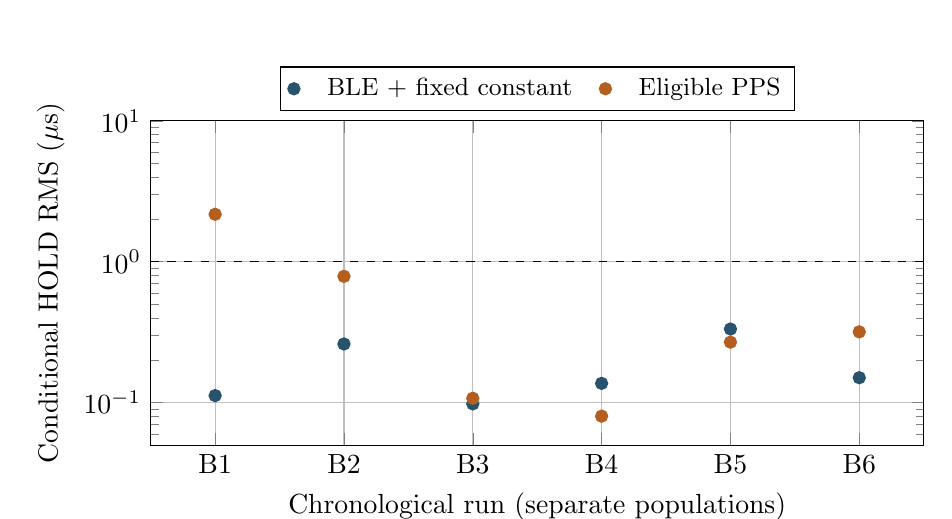
\begin{tikzpicture}\begin{semilogyaxis}[width=.94\linewidth,height=5.7cm,ymin=.05,ymax=10,xmin=.5,xmax=6.5,xtick={1,2,3,4,5,6},xticklabels={B1,B2,B3,B4,B5,B6},ylabel={Conditional HOLD RMS ($\mu$s)},xlabel={Chronological run (separate populations)},legend style={column sep=.8em,font=\small,at={(.5,1.03)},anchor=south,legend columns=2},grid=major]
\addplot[studyblue,thick,only marks,mark=*] coordinates {(1,0.1123315811) (2,0.2609765626) (3,0.09809248071) (4,0.1371132009) (5,0.3332209654) (6,0.1503965518)};\addlegendentry{BLE + fixed constant}
\addplot[studyorange,thick,only marks,mark=*] coordinates {(1,2.173739217) (2,0.7881964524) (3,0.1075357615) (4,0.08025926738) (5,0.2689882618) (6,0.3181796152)};\addlegendentry{Eligible PPS}
\addplot[black,dashed,forget plot] coordinates {(.5,1)(6.5,1)};
\end{semilogyaxis}\end{tikzpicture}
% END GENERATED conditional-rms
\caption{Conditional HOLD RMS, keeping each run and endpoint separate. The dashed line is 1 $\mu$s. BLE observations have the unequal coverage shown in Table~\ref{tab:precision}; the PPS series samples local fractional phase once per second. The two endpoints need not share errors or missingness.}\label{fig:rms}
\end{figure}

The most misleading interpretation would be to assign B1's 112 ns BLE RMS to all 202.5 s. Its last valid HOLD BLE capture occurred at 44.258 s, and 156 of its 200 expected HOLD-second bins had no valid BLE score. Its PPS witness continued through the HOLD population and showed 2174 ns RMS and 4762 ns maximum absolute phase. B4 likewise had only ten occupied bins of 100, ending its valid BLE observation near 9.258 s, despite its 137 ns conditional BLE RMS. B2, B5 and B6 had 284, 86 and 285 unoccupied bins, respectively. B3 occupied all 100 bins, but occupancy still does not provide continuous-time metrology. BLE absence truncates what BLE can say; the PPS observation contributes separate evidence rather than filling the missing BLE samples.

There were 1414 recorded PPS edges across the six whole-run intervals: 1400 in HOLD and 14 in LISTEN. All 1400 recorded HOLD edges were eligible. Of the 14 LISTEN edges, ten were ineligible and four eligible; these are excluded from Table~\ref{tab:precision}'s HOLD calculation. Reason and reference flags remain in the supplement. We do not discard those ten from the overall observation population or assign them zero phase error.

\subsection{Fit turnover and acquisition inheritance}
Only B3 selected at least 16 new pairs. Its generation advanced 26 to 42, replacing the initial 16-pair fit history. The sixteenth selected pair completed at 92.330255875 s into the 102.5 s schedule. The remaining 10.169744125 s contained 149 causal HOLD BLE scores, with normalized RMS 144.780649 ns. This is brief post-turnover observation; it is not a steady-state sleep or sparse-maintenance qualification.

The other five runs retained at least part of their acquisition history. B4's single selected pair and low PPS RMS are especially clear reasons not to credit cadence with maintaining the map: a favorable initial frequency estimate may dominate a short observation. Different starting fits, availability, elapsed history and uncontrolled temperature prevent a causal ranking of 5, 10 and 20 s HOLD. Two randomized repetitions per duration cannot characterize tails, aging or thermal changes. Thousands of samples within a run do not supply thousands of independent run replications.

\section{A scheduling model with explicit information costs}\label{sec:scheduling}
\subsection{Complete-pair availability}
For a window of width $W$, let $A$ denote availability of an admitted source and retained transport, $J$ the offset of the target RX relative to its prediction, and $D$ its reference completion latency. With an early guard $g$, one targeted complete pair requires
\begin{equation}
 A,\qquad -g\le J,\qquad g+J+D<W.\label{eq:probability}
\end{equation}
The probability of those joint events depends on source availability, RF delivery, controller scheduling and latency; independence is not assumed. PC117 establishes a finite empirical aperture for selected events. Its empty windows establish that phase positioning does not solve availability. An always-available synthetic source and an outage-injected source are both needed to estimate different terms of this model.

Suppose future measurements support an availability probability $p$ for one usable refresh per cycle and independent, stationary cycles. Then the expected cycles to collect 16 refreshes would be $16/p$. At the hypothetical $p=0.8$ and $C=5.125$ s, the mean turnover time would be 102.5 s. That arithmetic explains why a 20-window pilot can end just after turnover. It is not a confidence model for this campaign: its long empty sequences and changing source conditions violate the independence premise. Reporting a pooled $42/120$ success rate as a portable $p$ would hide both run variation and outages.

A controller should budget maximum age since the \emph{last complete selected update}, not just time since the most recent scheduled wake. After $m$ consecutive failures, the map's information age can approach $(m+1)C$, while the nominal training fraction stays unchanged. Age, fit span, count of genuinely new pairs, ancestry and uncertainty must be state variables. They cannot be replaced by a low sample RMS.

\subsection{Guard widening and wake uncertainty}
A proposed wake lead must cover hardware start, transport readiness and the early side of timing uncertainty. One conservative decomposition is
\begin{equation}
 g(H)\ge t_{\mathrm{ready,max}}+j_{\mathrm{wake,max}}+
 q_{\mathrm{align,max}}+\rho_{\mathrm{rel,max}}H+g_{\mathrm{margin}},\label{eq:guard}
\end{equation}
where relative drift is expressed in time per second. The late side and a chosen reference-latency bound or quantile must also fit: $W\ge g+J_{\mathrm{late}}+D_{\mathrm{budget}}$. A quantile gives a declared failure probability, not a hard guarantee. Correlation, oscillator transitions and controller work may invalidate an assumed tail model. PC117's 8 ms lead was an awake scheduling input, and its completion margins cannot calibrate $t_{\mathrm{ready}}$ or physical wake jitter.

Packet-event listening and application training are separate layers. If a future controller retains periodic synchronization, it might skip events and wake before selected ones; if that state is lost, scanning, synchronization and authenticated admission enter the acquisition budget. Bluetooth train management and application source permission must be verified with the pinned implementation. A 125 ms application gate must not be translated directly into a radio off/on command without proving bounded drain, timebase continuity and source validity.

\subsection{Precision targets and retained timebases}\label{sec:drift}
For sensitivity, assume a zero-mean independent initial phase error $\sigma_0$, wake alignment jitter $\sigma_w$, quantization error $\sigma_q$, and constant residual fractional-rate uncertainty $\rho$ expressed in ppm. A simple projected RMS model in microseconds is
\begin{equation}
 \sigma(H)=\sqrt{\sigma_0^2+\sigma_w^2+\sigma_q^2+(\rho H)^2},\qquad
 H_{\max}=\frac{\sqrt{T^2-\sigma_0^2-\sigma_w^2-\sigma_q^2}}{|\rho|}.\label{eq:drift}
\end{equation}
The second expression exists only for positive numerator budget and $\rho\ne0$. Persistent bias, covariance, frequency random walk and temperature dependence require additional terms or a different model. A conservative absolute-error analysis instead adds bounded initial error, accumulated bounded drift, quantization and wake errors. Neither expression's inputs are estimated by fitting away this campaign's residuals.

Table~\ref{tab:budget} uses illustrative $\sigma_0=0.1\us$, $\sigma_w=0.2\us$ and $\sigma_q=0$, with no unknown bias. The targets are \emph{instantaneous projected RMS at maximum age}, stronger than an average RMS over a HOLD with constant-rate error (whose age-squared average would be $H^2/3$). This distinction matters when selecting an application target. At 0.1 ppm residual uncertainty, the sub-1 $\mu$s example permits about 9.75 s; at 1 ppm it permits only 0.975 s. These are design sensitivities, not measured drift specifications for PC117 or sleep.

\begin{table}[t]\centering\small
\caption{Hypothetical maximum information age (s) from Eq.~\ref{eq:drift}. Assumed independent zero-mean errors: $\sigma_0=0.1\us$, $\sigma_w=0.2\us$, no quantization or bias. No entry is a qualified operating interval.}\label{tab:budget}
\begin{tabular}{rrrr}\toprule
Residual $\rho$ (ppm) & $T=1\us$ & $T=10\us$ & $T=100\us$\\\midrule
0.01 & 97.468 & 999.750 & 9999.975\\
0.1 & 9.747 & 99.975 & 999.997\\
1 & 0.975 & 9.997 & 100.000\\
10 & 0.097 & 1.000 & 10.000\\\bottomrule
\end{tabular}
\end{table}

\begin{figure}[t]\centering
% BEGIN GENERATED drift-model
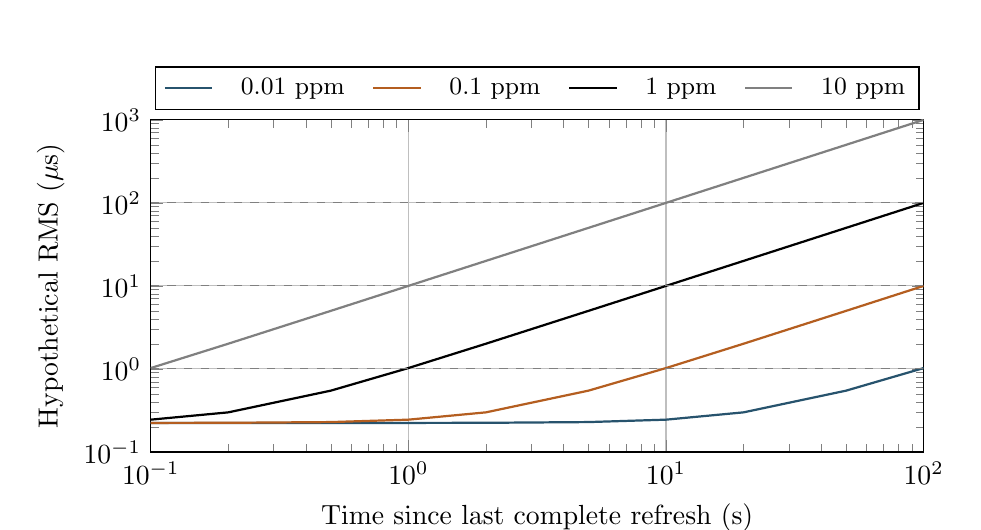
\begin{tikzpicture}\begin{loglogaxis}[width=.94\linewidth,height=5.8cm,xmin=.1,xmax=100,ymin=.1,ymax=1000,xlabel={Time since last complete refresh (s)},ylabel={Hypothetical RMS ($\mu$s)},legend style={column sep=.8em,font=\small,at={(.5,1.03)},anchor=south,legend columns=4},grid=major]
\addplot[studyblue,thick] coordinates {(0.1,0.2236090338) (0.2,0.2236157418) (0.5,0.2236626925) (1,0.2238302929) (2,0.2244994432) (5,0.2291287847) (10,0.2449489743) (20,0.3) (50,0.5477225575) (100,1.024695077)};\addlegendentry{0.01 ppm}
\addplot[studyorange,thick] coordinates {(0.1,0.2238302929) (0.2,0.2244994432) (0.5,0.2291287847) (1,0.2449489743) (2,0.3) (5,0.5477225575) (10,1.024695077) (20,2.01246118) (50,5.004997502) (100,10.00249969)};\addlegendentry{0.1 ppm}
\addplot[black,thick] coordinates {(0.1,0.2449489743) (0.2,0.3) (0.5,0.5477225575) (1,1.024695077) (2,2.01246118) (5,5.004997502) (10,10.00249969) (20,20.00124996) (50,50.0005) (100,100.00025)};\addlegendentry{1 ppm}
\addplot[gray,thick] coordinates {(0.1,1.024695077) (0.2,2.01246118) (0.5,5.004997502) (1,10.00249969) (2,20.00124996) (5,50.0005) (10,100.00025) (20,200.000125) (50,500.00005) (100,1000.000025)};\addlegendentry{10 ppm}
\addplot[dashed,gray,forget plot] coordinates {(.1,1)(100,1)};
\addplot[dashed,gray,forget plot] coordinates {(.1,10)(100,10)};
\addplot[dashed,gray,forget plot] coordinates {(.1,100)(100,100)};
\end{loglogaxis}\end{tikzpicture}
% END GENERATED drift-model
\caption{Hypothetical retained-map RMS versus information age, using Table~\ref{tab:budget}'s assumptions. Dashed levels are 1, 10 and 100 $\mu$s. Curves express sensitivity to residual frequency uncertainty; they are not fits to the BLE or PPS records.}\label{fig:drift}
\end{figure}

If timing is handed to a 32.768 kHz counter with an otherwise unobserved uniform tick phase, one tick is 30.5176 $\mu$s and the illustrative centered quantization RMS is $30.5176/\sqrt{12}=8.8097\us$. A sub-1 $\mu$s target then has no budget even at zero HOLD; a sub-10 $\mu$s target becomes tight. At 1 ppm, the same illustrative model permits about 4.726 s for the 10 $\mu$s target and 99.611 s for 100 $\mu$s. This is not an unavoidable floor for all architectures: a validated HF/LF cross-timestamp and phase interpolation could reduce uncertainty. It is a warning that retained RAM and coarse time alone do not preserve the awake map's fine counter phase.

\subsection{Repeated short listens versus longer bursts}
A complete timing pair occupies two logical events and associated compute. If its reference takes about 70 ms to become available, a very short listen can capture the first event but miss the second. Several short listens may provide independent chances, or repeatedly miss the same event because their phase is wrong. A longer burst can supply multiple fit pairs, amortize startup and span source jitter, but increases active duration and can overrepresent one short thermal epoch.

Under an illustrative independent-attempt model, three tries at $p=0.5$ yield $1-(1-p)^3=0.875$ probability of at least one usable pair. Correlated outages can instead make all three fail together. For example, four 125 ms listens contain 500 ms of nominal listening; one continuous 562.5 ms burst costs 62.5 ms more listening but needs three fewer wake transitions. Ignoring sleep-power differences and changed availability, at 15 mW listening power those extra 62.5 ms cost 0.9375 mJ. Four listens cost more when each additional transition costs over 0.3125 mJ. This example does not assume equal information, equal latency, or equal precision: those must be measured. It supplies a falsifiable crossover calculation rather than a preference for a particular cadence.

A candidate adaptive policy would use brief listens while the source is healthy and the map young, lengthen a bounded burst after incomplete pairs, and reacquire after an explicit information-age or ancestry boundary. It must preserve all failed attempts and stop claiming valid output when permission or uncertainty expires. Its guard and burst ceilings must be predeclared; success must not be manufactured by silently extending the window until a reference arrives.

\section{Energy model and sensitivity}\label{sec:energy}
No current trace or radio-airtime measurement was collected. To estimate possible savings, define a fixed proposed cycle $C=H+W$, a listen interval $W$, startup interval $t_s$ and compute interval $t_c$ inside the remaining cycle, with sleep time $C-W-t_s-t_c\ge0$. Powers $P_l,P_s,P_{\mathrm{start}},P_c$ refer to a selected metering boundary. Let $E_w$ be additional transition energy not already included in those intervals, $E_r$ the incremental reacquisition energy and $r$ its expected events per cycle. Let $P_a$ represent continuously active auxiliary loads omitted from the other powers. Then
\begin{align}
 E_{\mathrm{cycle}}={}&P_s C+(P_l-P_s)W+(P_{\mathrm{start}}-P_s)t_s\nonumber\\
 &+(P_c-P_s)t_c+E_w+rE_r+P_a C,\label{eq:energy}\\
 \overline{P}={}&E_{\mathrm{cycle}}/C.\label{eq:pavg}
\end{align}
Powers in mW and times in s give energy in mJ. Terms must be disjoint to avoid counting oscillator startup or compute twice. $E_r$ includes incremental event energy under the same time-accounting convention; if reacquisition lengthens the cycle, its duration must also enter the denominator and availability calculation. With reacquisition once every $K$ cycles, $r=1/K$. A continuous-listen comparison is $P_l+P_a$ only if it supplies the same service and shares the same metering boundary.

For an explicit illustration, choose $P_l=15$ mW, $P_s=0.03$ mW, $P_{\mathrm{start}}=10$ mW for $t_s=5$ ms, $P_c=5$ mW for $t_c=2$ ms, $E_w=0.05$ mJ, $E_r=10$ mJ and $r=0.01$. None is a fitted or measured board value. The overhead beyond the sleep/listen mixture is 0.20979 mJ per cycle. Table~\ref{tab:power} shows the resulting arithmetic. A permanently active 20 mW auxiliary load limits relative reduction to about 42\%, despite the small scheduled training fraction. A GNSS witness or USB logging configuration may similarly dominate a board measurement; it must be measured rather than assigned one of these example values.

\begin{table}[t]\centering\small
\caption{Hypothetical power using the explicit central scenario. Each power includes the stated auxiliary load; reduction is relative to $15+P_a$ mW. These values are neither datasheet predictions nor measured T096 savings.}\label{tab:power}
\begin{tabular}{rrrrrrr}\toprule
 & \multicolumn{2}{c}{$P_a=0$ mW} & \multicolumn{2}{c}{$P_a=5$ mW} & \multicolumn{2}{c}{$P_a=20$ mW}\\
$H$ (s) & mW & Reduction & mW & Reduction & mW & Reduction\\\midrule
5 & 0.4361 & 97.09\% & 5.4361 & 72.82\% & 20.4361 & 41.61\%\\
10 & 0.2355 & 98.43\% & 5.2355 & 73.82\% & 20.2355 & 42.18\%\\
20 & 0.1334 & 99.11\% & 5.1334 & 74.33\% & 20.1334 & 42.48\%\\\bottomrule
\end{tabular}
\end{table}

\begin{figure}[t]\centering
% BEGIN GENERATED energy-model
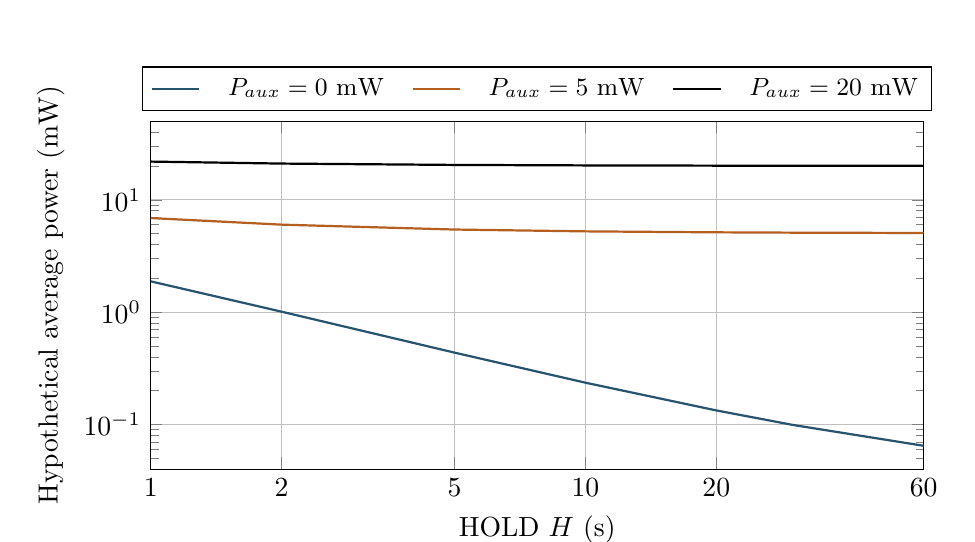
\begin{tikzpicture}\begin{axis}[width=.94\linewidth,height=6cm,xmode=log,ymode=log,xmin=1,xmax=60,xtick={1,2,5,10,20,60},xticklabels={1,2,5,10,20,60},ymin=.04,ymax=50,xlabel={HOLD $H$ (s)},ylabel={Hypothetical average power (mW)},legend style={column sep=.8em,font=\small,at={(.5,1.03)},anchor=south,legend columns=3},grid=major]
\addplot[studyblue,thick] coordinates {(1,1.879813333) (2,1.009312941) (5,0.4360565854) (10,0.2355348148) (20,0.1334057143) (30,0.09908016598) (60,0.06461189189)};\addlegendentry{$P_{aux}=0$ mW}
\addplot[studyorange,thick] coordinates {(1,6.879813333) (2,6.009312941) (5,5.436056585) (10,5.235534815) (20,5.133405714) (30,5.099080166) (60,5.064611892)};\addlegendentry{$P_{aux}=5$ mW}
\addplot[black,thick] coordinates {(1,21.87981333) (2,21.00931294) (5,20.43605659) (10,20.23553481) (20,20.13340571) (30,20.09908017) (60,20.06461189)};\addlegendentry{$P_{aux}=20$ mW}
\end{axis}\end{tikzpicture}
% END GENERATED energy-model
\caption{Hypothetical average power from Eq.~\ref{eq:energy}, with the central assumptions and three constant auxiliary loads. All curves presume a sleep-capable implementation and the stated overhead; none describes the measured awake PC117 power. Longer HOLD also increases drift exposure and the cost of missing refreshes.}\label{fig:power}
\end{figure}

The supplement sweeps broader, explicitly assumed corners: sleep power 0.003--1 mW; listening power 5--30 mW; extra wake energy 0.001--1 mJ; startup 0.1--50 ms at 5--30 mW; compute 0.1--20 ms at 1--20 mW; and reacquisition 1--100 mJ at zero to 0.1 expected events per cycle. Combining all low-overhead choices and all high-overhead choices gives 0.125--4.211 mW at 5 s HOLD, 0.0648--2.625 mW at 10 s and 0.0341--1.818 mW at 20 s before auxiliary loads. These corners are sensitivity scenarios, not confidence intervals, component specifications or a validated plausible range for the assembled board. Reacquisition stalls or a permanently running oscillator can produce larger consumption and unavailable output.

A break-even statement is more portable than an example saving. Let $\Delta E$ be all incremental startup, compute, transition and expected reacquisition energy beyond the listen/sleep mixture. For an otherwise equivalent continuous-listen baseline,
\begin{equation}
 (P_l-P_s)(C-W)>\Delta E\label{eq:break}
\end{equation}
is required for positive energy reduction. For a desired relative reduction $s$ including auxiliaries, the available per-cycle overhead budget is
\begin{equation}
 \Delta E\le (1-s)(P_l+P_a)C-P_sC-(P_l-P_s)W-P_aC.\label{eq:budgetenergy}
\end{equation}
A negative right-hand side means the requested reduction is impossible under those assumed loads even with free wake transitions. Datasheet SoC currents cannot supply these board-level terms without a measurement boundary, regulator efficiency, board leakage and device-state accounting. Energy per delivered valid timing second, and the fraction of scheduled service seconds that remain valid, should accompany mean power; a source that uses little energy while never producing usable time is not a successful optimization.

\section{Implementation alternatives and a physical test protocol}\label{sec:future}
\subsection{Three distinct retention classes}
\emph{Retained precision counter, CPU idle.} Preserve the exact counter and affine map, allow CPU idle between events, and determine whether radio/controller and peripherals can be gated while the precision timebase remains alive. This is the closest extension of the awake pilot. Its minimum current may still be dominated by HF-clock or peripheral requirements.

\emph{HF stopped, LF counter retained.} Cross-timestamp the high-resolution counter and an independently running LF counter before suspension and after wake. Preserve overflow accounting, frequency estimate and uncertainty across the handoff. Restart HF early enough for stable capture, verify oscillator source changes, and admit timing only after the reconstructed map's uncertainty is acceptable. Unmeasured phase transfer is a new error term; copying the old slope into a restarted counter is insufficient.

\emph{System OFF or physical cold start.} Treat wake as a reset with explicitly documented retained memory and reset cause. On nRF52840, System OFF stops LFCLK; RAM retention supplies state without a running internal LF elapsed-time measurement. An external always-on reference or a fresh acquisition would be needed for an elapsed-time claim across that interval. Cold boot also includes bootloader, oscillator, controller, train discovery, admission and estimator costs. The earlier 0.54--0.66 s first-map brackets and this study's 2 s priming budget omit those physical costs.

These alternatives are proposed experiments. A Nordic sleep implementation, wake processor, power-meter trace and physical cold-start precision result remain future work. Changing a Zephyr configuration symbol alone cannot establish any of them.

\subsection{Predeclared follow-on experiment}
A practical protocol should make energy and information failure visible together:
\begin{enumerate}
\item Freeze one exact source/firmware/board configuration and its public build identity. Record placement, antenna orientation, supply, ambient and device temperature, source policy and oscillator sources. Keep enrollment and exact device bindings in local records. Use separately authorized hardware ownership and recovery procedures for the selected receiver.
\item Measure a continuous awake control, retained-counter idle, radio-off/reacquire, HF-to-LF retained sleep, and physical reset as separate populations. Do not pool across them or infer one from another. Run a deterministic healthy source first; then repeat with predeclared source outages and returns. Distinguish absent source, unauthenticated/rejected source, missed RX and late reference.
\item Meter the whole board at a declared supply boundary with a calibrated current/voltage instrument. Choose bandwidth and sample rate from the shortest transition of interest, resolve individual packet/start events where possible, and verify integration against a known load. Capture synchronized hardware markers for request, actual radio closure, sleep entry, wake interrupt, stable HF clock, controller ready, first RX, first completed reference, first map, first authorized output and first independently acceptable phase. Characterize marker overhead.
\item Use an independent phase instrument or calibrated reference chain with explicit uncertainty, PPS association and path delay. Capture output edges if output precision is claimed. Retain the local PPS observer as a separate stream; it does not substitute for calibrated output metrology. Meter the deployment without a USB/GNSS witness load separately from the instrumented configuration, while preserving a valid observation path.
\item Randomize 125, 250, 500 and 2000 ms windows and 1, 5, 10 and 20 s HOLD within each retention class. Include repeated short listens and equal-total-duration longer bursts with matched information-age ceilings. Use at least ten independently reacquired runs per selected condition as an initial design, then determine further sample size from run-level variability rather than treating packets as independent replicates. Record unstarted cases and all failed priming/reacquisition attempts.
\item Require at least three complete replacements of the 16-pair history before a separately declared steady observation interval, and retain the startup/turnover intervals as results. Extend the final interval to at least 30 minutes for promising conditions, with additional multi-hour thermal/source-loss trials as a separate stage. Do not stop a run when its RMS first looks favorable. Bound every wait and retry; a source outage must not create an unreported extension of the nominal energy cycle.
\item Predeclare sub-1, sub-10 and sub-100 $\mu$s RMS evaluations with maximum information age, available/eligible/unknown denominators, maxima and a separate calibrated-output criterion. Report per-age-bin bias-preserving RMS and run-level distributions. Freeze failure criteria for missed wakes, counter discontinuities, expired authority and phase excursions. For an initial screening gate, require at least 99\% of scheduled service-second bins to have qualified observations and valid service, with no unreported interval; that is a proposed gate, not a present result or a worst-case guarantee.
\item Integrate startup, listen, compute, idle, sleep and reacquisition energy from traces; report uncertainty and energy per valid service second. Compare against the equivalent-service awake control. Keep source, boot, capture and power epochs distinct, seal originals, and publish only reviewed sanitized exports with provenance.
\end{enumerate}
The 8 ms guard is a starting hypothesis in this protocol, not a mandated operating value. Sweep it against measured wake and RX uncertainty, include intentionally insufficient guards as negative controls, and preserve late completions. A successful phase-alignment test must not silently gain off-window information or extra listening time.

\section{Limits and interpretation}\label{sec:limits}
This is a one-receiver, finite-duration awake pilot, with two main runs per HOLD duration and no controlled source availability or thermal intervention. Randomizing order reduces a simple ordering confound but cannot identify cadence effects with changing initial fits and source conditions. No causal attribution of outages to placement, RF path, discovery scanning or one firmware mechanism follows from the record categories. PC117's management-scan isolation is a documented change, not proof of why earlier or current source absences occurred.

The observation paths have distinct limits. Causal BLE scores disappear with their source and depend on an inherited provisional bias correction. Local PPS provides longer support in these selected runs but measures fractional phase with unresolved absolute calibration and association; it does not resolve every instant or establish ordinary output authority. Complete recorded HOLD PPS eligibility is not a claim of independent UTC traceability. The frozen experimental map is not an authorized indefinitely valid time service.

The energy curves are equations evaluated under declared assumptions. They do not transfer Nordic typical current to the board, identify battery life, measure RF airtime, or establish a wake-latency distribution. The source and phase anchor survived in an awake receiver; physical sleep may change all relevant error and acquisition terms. The single brief post-turnover interval cannot establish stationary sparse refresh. The sanitized supplement allows independent recomputation from selected derived data; withheld raw physical records limit independent reconstruction of extraction, authentication and metrology.

\section{Conclusion}
The awake PC117 experiment shows that a fixed 125 ms training aperture can capture selected complete BLE timing pairs after 5--20 s gaps while retaining small conditional relative errors. It also exposes the decisive limits: 78 of 120 windows were empty, observation coverage collapsed in several runs, and only one run replaced its acquisition fit before the schedule ended. Those facts constrain the power hypothesis more strongly than a nominal training fraction alone.

Useful low-power timing will require demonstrated timebase retention, bounded complete-pair availability, explicit reacquisition behavior, calibrated phase observation and measured board energy under the same service requirement. The present result is an information-budget pilot and a reproducible set of models and tests for that next step.

\appendix
\section{Public supplement and reproduction}\label{app:reproduction}
The repository supplement is \code{evidence/power/2026-10-19/}. It contains 7326 derived BLE rows, 1414 PPS rows, six block summaries, 120 cycle summaries, 123 reduced HOLD audit states, nine priming outcomes, a selected protocol, separate earlier-context summaries, result recomputation and claim provenance. Numerical error and interval fields are unchanged except for shifting absolute hardware ticks to time relative to each scheduled start. Actual device, parent, root, boot and epoch identifiers are replaced with equality-preserving aliases; the private alias lookup is excluded.

No raw console or authentication envelopes, keys, enrolled images, factory bindings, private working files or private source history are included. Original evidence and derived datasets are CC BY 4.0, attributed to Jonathan Yantis; executable analysis and ordinary repository documentation are MIT. Cited third-party works retain their own terms.

From a public checkout with Python 3.9 or newer, run
\begin{quote}\small\ttfamily
python3 tools/verify\_power.py\\
python3 tools/verify\_power.py --out artifacts/power-rebuild
\end{quote}
The first command verifies public hashes, per-record normalization and eligibility, per-run counts/RMS, cycle bounds, map turnover, empty-window categories and embedded figure data. It performs no network, device or daemon operation. The second writes a fresh JSON recomputation and standalone PGFPlots figure sources. It requires a new output directory and never rewrites sealed inputs. The model results include the central power cases, declared sensitivity corners and both fine-counter and coarse-RTC drift budgets.

The manuscript is self-contained: its bibliography and vector figures are inline. With a public Tectonic installation, compile it using
\begin{quote}\small\ttfamily
tectonic --outdir artifacts/papers papers/ptob-power-scheduling-preprint.tex
\end{quote}
The first use may obtain a public TeX bundle. Ordinary numerical verification needs only the Python standard library and this checkout. A matching edition manifest records the PDF/source hashes, compiler identity, evidence cutoff and visual inspection. Recompilation may change PDF bytes across compiler/bundle versions; that does not change the evidence hashes.

\section{Claim boundaries and denominators}\label{app:claims}
\begin{longtable}{L{0.28\linewidth}L{0.31\linewidth}L{0.32\linewidth}}
\caption{Claim-to-evidence map. Machine-readable details are in the supplement's \code{claims.json}.}\label{tab:claims}\\\toprule
Claim & Public support & Boundary\\\midrule\endfirsthead
\toprule Claim & Public support & Boundary\\\midrule\endhead
42 refreshes, 78 empty windows & \code{cycles.csv}, \code{ble-records.csv}; 120 main windows & Aggregate accounting only; no pooled precision or stationary success probability.\\
69 empty windows without pairs; nine with RX but no selection & Per-cycle accepted RX and training flags & Absence does not identify its physical or protocol cause.\\
Frozen HOLD and fixed anchor & Reduced HOLD audit and audit receipt; 123 states including canary & Reduced export records the private raw audit result; raw-envelope reconstruction is unavailable publicly.\\
Selected RX and completion aperture & Relative ticks, offset and margin fields in every selected BLE row & Conditional selected-pair support; excluded/late/missing events remain outside it.\\
BLE HOLD RMS and coverage & All valid HOLD scores per block; raw and normalized errors; expected HOLD bins & Inherited fixed normalization; unknown bins remain unknown.\\
PPS HOLD RMS & 1400 eligible of 1400 recorded HOLD edges, separately per run & Independent local fractional phase; no calibrated UTC/output result.\\
Only B3 fit turnover & Training sequence, generations 26--42; 149 later HOLD scores & 10.169744125 s after sixteenth completion; no steady-state qualification.\\
Priming and earlier context & Nine PC117 attempts; separate PC112/115/116 context & Logical reset, retained awake receiver/counter; earlier populations never extend PC117 denominators.\\
Training fractions & $W/(W+H)$ and selected protocol & No measured RF airtime or energy.\\
Power and drift potential & Equations and executable explicit scenario inputs & Hypothetical, uncalibrated and conditional; physical sleep remains future work.\\\bottomrule
\end{longtable}

\section*{Acknowledgments and assistance}
Jonathan Yantis designed and conducted the experimental program and is responsible for the research claims. OpenAI Codex assisted with evidence curation, analysis implementation, literature checking, drafting and typesetting. This disclosure does not assign authorship to a model. No new hardware experiment or deployment accompanied preparation of this manuscript.

\begin{thebibliography}{10}\small
\bibitem{rbs} J. Elson, L. Girod, and D. Estrin, ``Fine-Grained Network Time Synchronization Using Reference Broadcasts,'' \emph{OSDI}, 2002. \url{https://www.usenix.org/conference/osdi-02/fine-grained-network-time-synchronization-using-reference-broadcasts}.
\bibitem{ftsp} M. Mar\'oti, B. Kusy, G. Simon, and \'A. L\'edeczi, ``The Flooding Time Synchronization Protocol,'' \emph{SenSys}, 2004. Author-hosted paper: \url{https://www.isis.vanderbilt.edu/sites/isis.vanderbilt.edu/files/bibcite_files/Maroti_M_11_3_2004_The_Floodi_0.pdf}.
\bibitem{btcore} Bluetooth SIG, \emph{Core Specification 6.0}, Vol. 6, Part B, especially Secs. 4.2.4, 4.4.2.12 and 4.4.5.1. \url{https://www.bluetooth.com/wp-content/uploads/Files/Specification/HTML/Core-60/out/en/low-energy-controller/link-layer-specification.html}. Accessed 19 October 2026; cited edition is explicit, not an assertion of the latest edition.
\bibitem{nordicpower} Nordic Semiconductor, \emph{nRF52840 Product Specification}, ``POWER---Power supply,'' System ON/OFF, RAM retention and reset. \url{https://docs.nordicsemi.com/r/bundle/ps_nrf52840/page/power.html}. Accessed 19 October 2026.
\bibitem{nordicclock} Nordic Semiconductor, \emph{nRF52840 Product Specification}, ``CLOCK---Clock control,'' HFCLK/LFCLK sources and System OFF behavior. \url{https://docs.nordicsemi.com/r/bundle/ps_nrf52840/page/clock.html}. Accessed 19 October 2026.
\bibitem{nordicrtc} Nordic Semiconductor, \emph{nRF52840 Product Specification}, ``RTC---Real-time counter,'' clock source and resolution. \url{https://docs.nordicsemi.com/r/bundle/ps_nrf52840/page/rtc.html}. Accessed 19 October 2026.
\bibitem{zephyrsystem} Zephyr Project, ``System Power Management,'' official documentation, residency and wake-source requirements. \url{https://docs.zephyrproject.org/latest/services/pm/system.html}. Accessed 19 October 2026; these architectural notes do not certify support in the pinned firmware build.
\bibitem{zephyrruntime} Zephyr Project, ``Device Runtime Power Management,'' official documentation. \url{https://docs.zephyrproject.org/latest/services/pm/device_runtime.html}. Accessed 19 October 2026.
\bibitem{supplement} J. Yantis, \emph{PToB awake information-budget pilot: selected PC117 derived evidence and scheduling models}, 19 October 2026 research-draft supplement. Repository supplement and edition receipt identified in Appendix~\ref{app:reproduction}. Public repository: \url{https://github.com/yantisj2/PToB}. This locally prepared edition has not been pushed or submitted; use its manifest and local commit to identify it.
\end{thebibliography}
\end{document}
